\documentclass[12pt,a4paper]{article}

\usepackage[utf8]{inputenc}
\usepackage{lmodern}
\usepackage[T1]{fontenc}
% paysage
% \usepackage[landscape]{geometry}
\usepackage{lscape}
\usepackage{graphicx}
% \graphicspath{ {images/} }

% headers footers
\usepackage{fancyhdr}
\pagestyle{fancy}

% référencer la dernière page
\usepackage{lastpage}

% pdf
\usepackage{pdfpages}

% francais
\usepackage[frenchb]{babel}
% math
\usepackage{amssymb}

\usepackage{multicol}
\usepackage{url}

\usepackage{multido}
\usepackage[utf8]{inputenc}
% \usepackage{lmodern}
\usepackage[T1]{fontenc}

\usepackage[sfdefault]{AlegreyaSans} %% Option 'black' gives heavier bold face
%% The 'sfdefault' option to make the base font sans serif
% \renewcommand*\oldstylenums[1]{{\AlegreyaSansOsF #1}}


\usepackage{multicol}
\usepackage[frenchb]{babel}
% \usepackage{pstricks,pst-plot,pst-node}
% \usepackage{pstricks-add}
\usepackage{pst-circ}
\usepackage{pst-magneticfield}
\usepackage{pst-electricfield}
\usepackage{graphicx}
\usepackage{amsmath,amsfonts,amssymb}
\usepackage{titlesec} 
\usepackage{float}
\usepackage{textcomp}
\usepackage{amssymb}
\usepackage[toc,page]{appendix}
\usepackage{listings} 

\lstset{language=Matlab}
\usepackage{lipsum}
\usepackage{enumerate}


%Numerotation par section des équations
\usepackage{amsmath}

\usepackage{tabularx}
\usepackage{longtable}

%------------------------------inclue les références
% \usepackage[nottoc, notlof, notlot]{tocbibind}
%\usepackage{biblatex}
% \usepackage{csquotes}

%\usepackage{etoolbox}
% \patchcmd{\chapter}{\thispagestyle{plain}}{\thispagestyle{fancy}}{}{}
\title{
	\Huge\textsc{Geographic coordinates}
}
\author{Mohamed Thebti} 

\begin{document}
% retrait de la première ligne d'un paragraphe
\setlength{\parindent}{0mm}

\fancyhead[R]{\slshape \leftmark}
\fancyhead[L]{\slshape 3D printing techniques}
%\fancyhead[LE,RO]{\slshape \rightmark}
% \fancyhead[LO,RE]{\slshape \leftmark}

% \fancyfoot[C]{Travail de Master}
\fancyfoot[L]{\slshape Mohamed Thebti}
\fancyfoot[C]{}
\fancyfoot[R]{\thepage}

\maketitle
\newpage

\tableofcontents

\newpage



\section{Introduction}

The objective of this report is record the techniques used in 3D printing. These are useful to make sure the designed part is printed as intended, without wasting time and resources. 


% 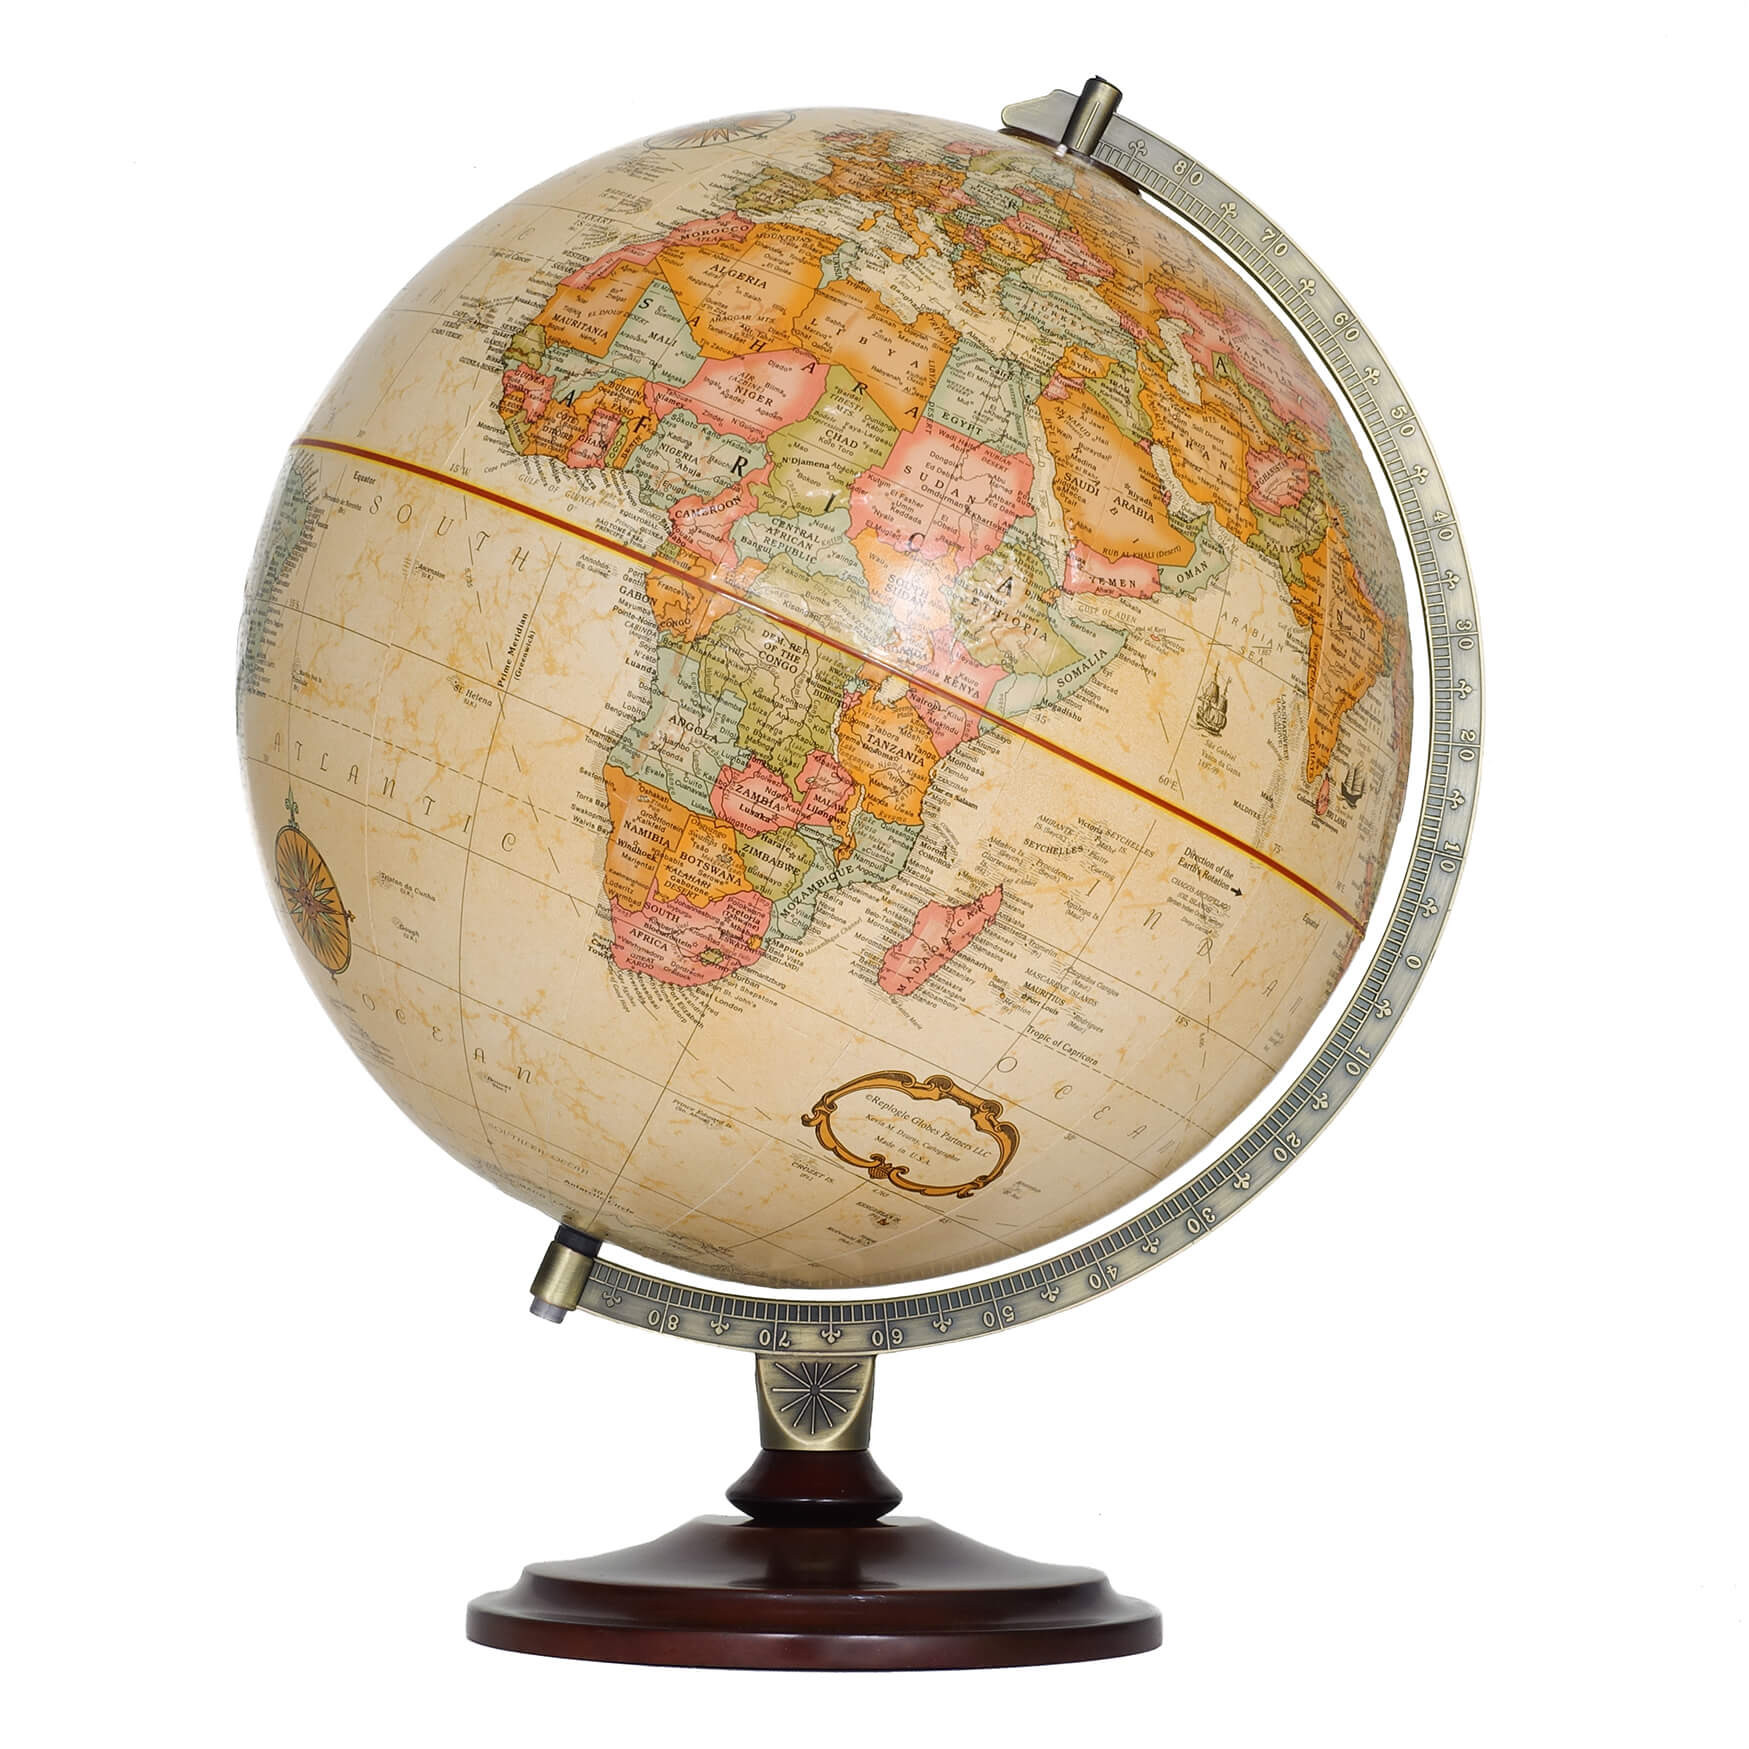
\includegraphics[scale=.2]{oxford-2021-01.jpg}

\newpage
\section{Techniques}
Prefabricated parts PFP /premanufactured parts PMP

Instead of creating the same parts again and again, design the components and make them easily modifiable.
for example, combine 2 parts to create a third one, which is useful in an other application. Then add them to the system in the assembly
Example : threads : try the smallest possible size, for example M3 to M20. 

Test them with small parts and check the tolerances. 
The next step is to prepare small parts ready to be added to system parts. The final step is the merge the bodies. 


table

\begin{table}[ht]
	\caption{Holes and threaded holes} % title of Table
	\centering % used for centering table
	\begin{tabular}{c c c} % centered columns (4 columns)
		\hline\hline %inserts double horizontal lines
		Screw & Threaded hole diameter & Bore Hole (clearance) \\ [0.5ex] % inserts table
		%heading
		\hline % inserts single horizontal line
		M3 & 2.8 & 3.2 \\ % inserting body of the table
		4 & 35 & 144 \\
		5 & 45 & 300 \\ [1ex] % [1ex] adds vertical space
		\hline %inserts single line
	\end{tabular}\label{table:nonlin} % is used to refer this table in the text
\end{table}

Clearance
To fix two part together, a clearance is needed.
When two parts must be assembled together, a clearance of 0.1mm is enough. Then use the glue to fix the assembly. 



\begin{table}[ht]
	\caption{Nonlinear Model Results} % title of Table
	\centering % used for centering table
	\begin{tabular}{c c c c} % centered columns (4 columns)
		\hline\hline %inserts double horizontal lines
		Case & Method\#1 & Method\#2 & Method\#3 \\ [0.5ex] % inserts table
		%heading
		\hline % inserts single horizontal line
		1 & 50 & 837 & 970 \\ % inserting body of the table
		2 & 47 & 877 & 230 \\
		3 & 31 & 25 & 415 \\
		4 & 35 & 144 & 2356 \\
		5 & 45 & 300 & 556 \\ [1ex] % [1ex] adds vertical space
		\hline %inserts single line
	\end{tabular}\label{table:nonlin} % is used to refer this table in the text
\end{table}



\begin{equation}
	Length_{lattitude}(\phi) = 111132.92-559.82 \cdot cos(2 \cdot \phi)+1.175*cos(4 \cdot \phi)-0.0023 \cdot cos(6 \cdot \phi)= ... [m/degree]
\end{equation}
 1 degree longitude at latitude phi
\begin{equation}
	Length_{longitude}(\phi) =
	111412.84-93.5 \cdot cos(3 \cdot \phi)+ 0.118 \cdot cos(5 \cdot \phi)= ... [m/degree]
\end{equation}

\newpage
\section{Schéma cinématique}


\subsection{Vecteurs positions}
origine : centre de rotation verticale se trouvant sous les pâles principales.
\medbreak
position  des pâles principales ($pp$) : vecteur verticale
\medbreak
position de l'hélice arrière : 
vecteur allant de l'origine vers l'hélice ($h$) arrière. 


\newpage
\section{Angular momentum}

\subsection{Formula}
\begin{equation}
\vec{L}=\vec{OA} \otimes \vec{P}=\vec{r} \otimes \vec{P}=\vec{r} \otimes m \cdot \vec{v}=\vec{I} \otimes \vec{\omega}
\end{equation}
$\vec{L}$ : Angular Momentum [$kg \cdot \frac{m^2}{s}$]\\
$\vec{OA}$ and $r$: position of the mass [$m$] according to a referance\\
$\vec{P}$ : linear momentum [$kg\cdot \frac{m}{s}$]\footnote{$\vec{L}$ is perpendicular to both $\vec{P}$ and $\vec{r}$}\\
$\vec{v}$ : velocity [$\frac{m}{s}$]
$I$ : moment of inertia [$m^2 \cdot kg \cdot$]\\
$\omega$ : angular speed [$\frac{rad}{s}$]

Torque : 
\begin{equation}
M = \frac{d\vec{L}}{dt}=\frac{d(\vec{I} \otimes \vec{\omega})}{dt}
\end{equation}
\medbreak
if we consider a particule of mass $m$, $\vec{r}$ is the position of the center of mass.
If it is a solid object, $L$ is first computed according to the axis of rotation of the object : 
\begin{equation}
\vec{L}_{ar}=\vec{I}_{ar} \otimes \vec{\omega}_{ar}
\end{equation}
To compute the angular moment according to an other axis of rotation (new referance), we use the Huygens-Steiner theorem (or the Parallel axis theorem) : 
\begin{equation}
\vec{L}_{0}=\vec{I}_{0} \otimes \vec{\omega}_{cm}\\
\end{equation}
\begin{equation}
\vec{I}_{0} = \vec{I}_{ar} + m\cdot d^2
\end{equation}
with $d$ the distance between the axis of rotation of the object and the new referance. 
\subsection{Condition of stability}

Main rotor(s):
\begin{equation}
\vec{L}_{mr}=\vec{r}_{mr} \otimes m_{mr} \cdot \vec{v_{mr}}=\vec{I_{mr}} \otimes \vec{\omega_{mr}}
\end{equation}


Rear rotor : 
\begin{equation}
\vec{L}_{rr}=\vec{r}_{rr} \otimes m_{rr} \cdot \vec{v_{rr}}=\vec{I_rr} \otimes \vec{\omega_{rr}}
\end{equation}

assurer la stabilité lors du vol: les moments cinétiques doivent s'annuler. (poser la formule et résoudre)
\begin{equation}
\vec{L_{mr}}=\vec{L_{rr}}
\end{equation}

or

The generated torque is compensated : 
\begin{equation}
\sum \vec{M_{mr}}=\sum \vec{M_{rr}}
\end{equation}

find a relation between $\omega_{mr}$ and $\omega_{rr}$ -> determine the transmission ratio

\subsection{Pivots à droite et à gauche}
pour tourner à gauche ou doite, on ne doit plus satisfaire la condition de stabilité. le pilote utiliser le pédalier pour accélérer/ralentir l'hélice arrière. ainsi les moments cinétiques ne sont plus égaux.
\medbreak
calculer l'effet de rotation sur l'hélicoptère si l'hélice est accélérée/ralentie de 10,20,30,.. $\%$. mettre un tableau. calculer la vitesse de rotation dans ces cas-là. 


\begin{equation}
\begin{bmatrix}
0 \\
0\\
l_1
\end{bmatrix}_{R_{1}} \enspace
\vec{AB}_{R_{2}}=
\begin{bmatrix}
0 \\
l_2\\
0
\end{bmatrix}_{R_{2}} \enspace
\vec{BC}_{R_{3}}=
\begin{bmatrix}
l_3 \\
0\\
0
\end{bmatrix}_{R_{3}} \enspace
\vec{CD}_{R_{4}}=
\begin{bmatrix}
0 \\
0\\
-l_4
\end{bmatrix}_{R_{4}} \enspace
\end{equation}

\begin{itemize}
	\item
	\item 
	\item 
\end{itemize}


\medbreak

\medbreak

\medbreak

\medbreak




\begin{equation}
\begin{split}
\vec{OE}_R=\vec{OA}_R+\vec{AB}_R+\vec{B B_1}_R+\vec{B_1 C_1}_R+\vec{C_1 C}_R\\+\vec{C C_2}_R+\vec{C_2 D}_R+\vec{D D_1}_R+\vec{D_1 E}_R
\end{split}
\end{equation}

\begin{equation}
\begin{split}
\vec{OF}_R=\vec{OA}_R+\vec{AB}_R+\vec{B B_1}_R+\vec{B_1 C_1}_R+\vec{C_1 C}_R\\+\vec{C C_2}_R+\vec{C_2 D}_R+\vec{D D_1}_R+\vec{D_1 E}_R+\vec{E F}_R
\end{split}
\end{equation}

\begin{equation}
\begin{split}
\vec{OG}_R=\vec{OA}_R+\vec{AB}_R+\vec{B B_1}_R+\vec{B_1 C_1}_R+\vec{C_1 C}_R+\vec{C C_2}_R\\+\vec{C_2 D}_R+\vec{D D_1}_R+\vec{D_1 E}_R+\vec{E F}_R+\vec{F F_3}_R+\vec{F_3 G}_R
\end{split}
\end{equation}

\begin{equation}
\begin{split}
\vec{OH}_R=\vec{OA}_R+\vec{AB}_R+\vec{B B_1}_R+\vec{B_1 C_1}_R+\vec{C_1 C}_R+\vec{C C_2}_R+\vec{C_2 D}_R\\+\vec{D D_1}_R+\vec{D_1 E}_R+\vec{E F}_R+\vec{F F_3}_R+\vec{F_3 G}_R+\vec{G H}_R
\end{split}
\end{equation}

 
\section{Conclusion}


\end{document}